\section{The Rules of Poker}					% ----

% 2+ players.
% Each player has 2 cards only they can see.
% Round of betting, 3 community cards, round of betting, 1 community card, round of betting, 1 community card, round of betting. Winner takes pot/winners split pot.
% Description of a betting round.
% Some basic strategy.
% Mention the appendix A for more on the rules of poker.
% Mention the different variations of poker and why I chose \texas.


To help you better understand this project, I will now briefly explain the rules of Limit \texasp. 
%A more detailed explanation can be found at the end, in \hyperlink{rulesoftexas}{Appendix A}. 

There is a minimum of two players and usually no more than ten. At the start of each game, each player is dealt two cards, face down so that only they can see them. These cards are often called the hole cards.

Then there is a round of betting. In a round of betting, going clockwise through the group starting with the player to the left of the dealer, each player must choose to perform one of the following possible actions: they can fold, and drop out of the game; they can call, and place into the pot the current maximum bet; or they can raise, and increase the current maximum bet by a fixed amount. Note that calling when the current maximum bet is zero is usually called checking. The betting round continues until all players have either folded or matched the current maximum bet. 

Here is a quick example betting round between three players, Alice, Bob and Charlie:\\
\begin{center}
\begin{tabular}{c|c|c|c|c}
Player & Action & Amount in pot from & Total amount in pot & Current \\
 & & player before/after & before/after & maximum bet \\
\hline
Alice   & Check & \$0 / \$0 & \$0 / \$0 & \$0 \\
Bob     & Raise & \$0 / \$1 & \$0 / \$1 & \$1 \\
Charlie & Call  & \$0 / \$1 & \$1 / \$2 & \$1 \\
Alice   & Raise & \$0 / \$2 & \$2 / \$4 & \$2 \\
Bob     & Call  & \$1 / \$2 & \$4 / \$5 & \$2 \\
Charlie & Fold  & \$1 / \$1 & \$5 / \$5 & \$2 \\
\end{tabular}
\end{center}

After this round of betting, if at least two players are still in the game, three cards are dealt face up onto the table. There is another round of betting, another card on the table, another round of betting, a final card on the table and then a final round of betting. The four betting rounds are usually given the following names: preflop, flop, turn and river.

If all but one of the players folds then the remaining player takes all of the money in the pot. If the final betting round has ended and there are still two or more active players then there is a showdown; all active players show their cards and the player who can make the best poker hand wins the pot. It is also possible for multiple players to be able to make the same best poker hand. In this case, they will each take an equal share of the pot.

The best poker hand of each player is made up of the best combination of their two hole cards and the five cards on the table. The exact ranking of a poker hand is quite complicated and not really necessary to know for this project so I will not describe it in any more detail. All you need to know is that there are relatively fast algorithms for finding a numerical rank of a poker hand such that any better hand will have a higher rank, any worse hand will have a lower rank and any equal hand will have the same rank.

In Limit \texas, the small bet is the amount that one is allowed to increase the current maximum bet by (in the first two betting rounds). In the above example the small bet is \$1. In the last two betting rounds, the amount that one is allowed to increase the current maximum bet by is usually doubled (to \$2 in this example). To avoid any confusion, throughout this project the small bet will always be equal to \$1. Also there is a limit to how large the current maximum bet can be. The limit is usually four times the raise increment (so \$4 in the first two rounds of betting and \$8 in the last two). This puts a limit on length of the game. 

In the first round of betting (preflop) there is an additional rule. The player to the left of the dealer must place into the pot the small blind and the player to the left of that player must place into the pot the big blind. These blinds are similar to regular bets except they are not optional. The small blind and big blind are usually equal to one half of the small bet and one small bet respectively. The main purpose of the blinds is to get the betting going and prevent the players from all checking in the first round. Also, if no one else raises in the round then the player who put in the big blind is given the opportunity to raise.

There are a lot of complex rules regarding what to do when a player has run out of money but is still in the game. However these situations are very rare so I will not consider them.

There are many other varieties of poker including one where players can raise any amount they want. The reason I chose Limit \texas is because \texas is the most popular variety (and is the version I play) and because designing a No-Limit bot would have been too complicated. Also note that throughout the project, I will be referring to cash games as opposed to tournament games.

%Also note that throughout the project, I will always be talking about cash games as opposed to tournament games. The difference is that in cash games, winning \$10 will always be worth the same no matter how much money you already have. However in tournament games, winning \$10 when you only have \$5 left is worth more to you than if you had \$500 left. I chose to use cash games because it makes the strategy simpler and it means that I didn't have to simulate complete tournaments to get results. 



\section{\pap}									% ----

% What is it? It's not free. Graphical user interface. Provides the framework for playing poker bots against themselves. The statistics tracking abilities it has.
% Why other people use it and why I'm using it.
% The meerkat API.
% The flaws of \pa.
% The alternative to using \pap. Open Test Bed. Why I chose not to use it and if I regret my decision. What I would have done if I had used it. How the project would have been different if I had used it.
% Screenshots(?)


\pap \cite{pa} is a commercial program\footnote{It costs \$85 from the \pa website.} which provides a variety of useful and fun features for playing and analysing poker games. The two features that are relevant for this project are: the ability to play user created custom poker bots against a variety of existing poker bots; and the ability to record and analyse various statistics about the games played.

The \meer \cite{meer} provides the ability to create a plug-in bot which can play in the \pa program; all that is required is to create a Java class that implements a given interface.
% and you should be ready to go. 

I chose to use \pa because of the graphical user interface, because of its statistics tracking capabilities and because it was highly recommended. There were two alternatives. The first was to write the code for simulating the games myself. This would have been very difficult and would have taken too long.
The second possibility would have been to use opentestbed \cite{opentestbed}. Opentestbed is an open source implementation of the \meer for running poker games. In retrospect, I think it would have been better to use opentestbed. It was designed specifically for the purpose of testing poker bots and may have been easier to use. 
%However, I didn't use it.\footnote{Also it would be quite tricky to port my current program to it because my current program uses two important classes in the \meer which are not included in opentestbed.}

\begin{figure}[h!]
\centering
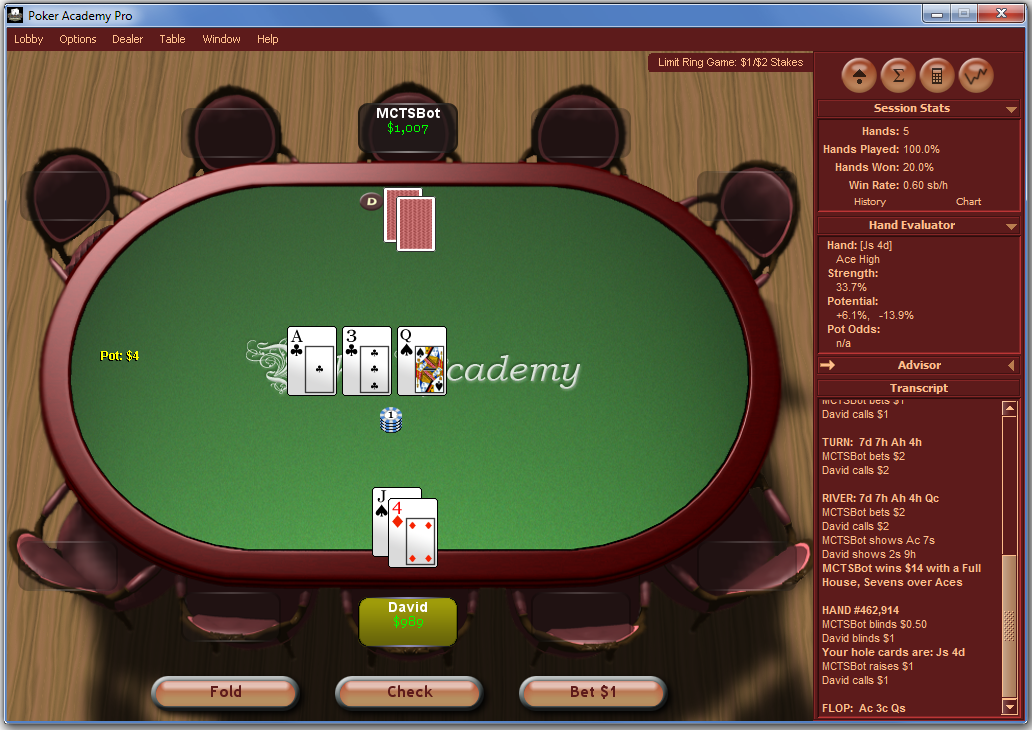
\includegraphics[width=144mm]{Screenshots/PAP1.png}
\caption{A screenshot of \pap.}
\end{figure}

%\begin{figure}[h!]
%\centering
%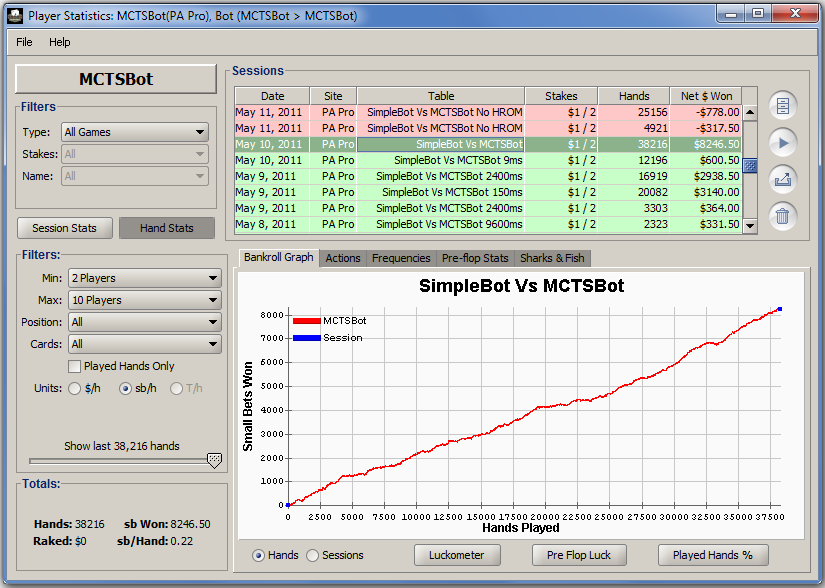
\includegraphics[width=144mm]{Screenshots/PAP2.png}
%\caption{Another screenshot of \pap.}
%\end{figure}



\section{\sbt}									% ----

% \sbt, what is it, how well does it play, and why am I using it?
% Where did it come from?
% The alternatives to using \sbt. I didn't want to compete.
% Attach the complete source code of \sbt?

 
%The source code for \sbt can be found in 
%Appendix \ref{app:sbsource}.
%\hyperlink{simplebotsourcecode}{Appendix B}.


\sbt is an example poker bot provided with the \meer. The important points to note about \sbt are:
\begin{itemize}
\item It only considers its own hole cards, the table cards, the amount in the pot and the number of active players.
\item It ignores the past actions of all players.
\item It is non-deterministic and has the ability to bluff.
\end{itemize}

\sbts playing ability is not comparable to that of an experienced human's, however it is good enough to provide a challenge for another poker bot. 

I chose to use \sbt as the opponent to test and evaluate my program against throughout the project. I did this because I needed an opponent to test against and I didn't want to be in competition with some of the really strong poker bots that have been in development for years. Thus, I settled on \sbt, a good enough opponent to provide a challenge but not so good that 
%I wouldn't be able to succeed.
I wouldn't stand a chance.

%The \sbt source code also helped me to understand some of the features of the \meer and was very useful when creating my program. 



\section{The Game Tree}							% ----

% This used to be in the imp.

% What is a game tree in general and why is it needed for the \mcts algorithm?
% What is it in this case, i.e. what are the nodes in the tree and what order/structure is there.
% Make a diagram of a game tree?
% Make distinction between the stored game tree and the full game tree.
% Choice nodes: Your turn, need to choose an action, root node is always a choice node.
% Opponent nodes: an opponent's turn, need to model them to see what they will do next.
% Chance nodes: Betting round has just finished and new cards are about to be drawn. Mention that there can be many possible children when three cards are to be drawn and how I got around it.
% Leaf nodes: The game has just ended. There are several possible cases.
% All opponents folded and you didn't, you win.
% You folded, you lose.
% You didn't fold and at least one other opponent is still in the game, need to guess result from table and betting history.
% Also mention at some point, not necessarily here, that I am modelling cash games not tournament play, and also that there is a limit of 4x the small bet per betting round.

% Make the distinction that I'm now talking about the actual implementation of the nodes rather than the general idea of nodes.
% Introduce the Node abstract class. 
% Stores several things needed by the \mcts algorithm including: visit count, expected value, std dev, etc.
% Mention all of the separate classes for the different nodes and say that more detail is coming in the next section.


%In this section I will explain what a game tree is and how it relates to poker and the MCTS algorithm. I will then go on to describe the different types of node found in the tree.

A game tree is a directed graph where each node represents a possible state in the game. An edge between nodes represents an action that transforms the parent node into the child node. The root node is the initial position and the leaf nodes represent positions in which the game has ended.
%are the final positions in which you either win, lose or draw \cite{gametree}.

For games which have perfect information and no random elements, it is possible to search the tree using the minimax algorithm. 
There are extensions to the minimax algorithm which allow it to deal with random elements (expectiminimax) and larger trees (alpha-beta pruning or limiting depth search combined with an evaluation function).
However, there are a few problems with these methods and they are not always suitable for poker. 

%However, this isn't practical in poker (and so you have to use something else, like MCTS).

%TODO: cite something for this?

%TODO: talk about minimax?

% Add some connecting scentence here?


In the poker game tree, there are several different types of node:
\begin{itemize}
\item Choice node, this is where the next action will be performed by the bot. It can choose to raise, call or fold and the children of this node will reflect the choice that was made.
\item Opponent node, this is where the next action will be made by one of the opponents. They can raise, call or fold. 
\item Chance node, this is where the current betting round has ended and one or more new cards are about to be dealt onto the table. This node can have either 46 or 47 children in the flop or turn stages, where one card is about to be dealt, or 50*49*48=117600 children in the preflop stage, where three cards are about to be dealt. 
\item Leaf node, this is where the game has ended. This node type has no children. There are three possible subtypes of this node:
	\begin{itemize}
	\item All opponents folded, this is where the bot is the only remaining player in the game; it wins by default. 
	\item Bot folded, this is where the bot has folded but other players are still in the game. The game might not necessarily have ended, however since the bot is no longer playing, there is no point in continuing.
	\item Showdown, this is where the bot and one or more other opponents are still playing and the final betting round has ended. In this case, it is not possible to say who wins because there is no way to tell what cards the opponents have. The result of the game has to be estimated from the strength of the best poker hand that the bot can make and the behaviour of the opponents up to this point.
	\end{itemize}
\end{itemize}

%For an example poker game tree between two players, see the following diagram.

%TODO: make diagram.





\section{\mcts}									% ----

% Briefly, what is a game tree?
% Very briefly, what is \mcts.
% Why is it appropriate here?
% The stages:
% Selection: Choose which node to explore. Need to have a good balance between exploration and exploitation. Several possible strategies to use here. Using opponent modelling here.
% Expansion: Generate the new nodes from the current node, generally trivial.
% Simulation: Very complicated part. Many possible strategies to use here. It is important that it is quick and easy to do. Simulate to completion, game cannot go on forever. Always call/others, using opponent modelling here.
% Backpropagation: Update the game tree. Two possible strategies both very similar.
% Repeat until finished.
% Again mention the project that I'm basing mine on.

\label{sec:mcts-prep}

%I will now describe the general \mcts algorithm. In the implementation chapter, I will go into more detail about how it relates to poker and about the specific strategies that I used.

The \mcts algorithm gradually builds up a subsection of the full game tree by starting at the root node and adding a new node in each iteration. The new nodes are not added at random though, the algorithm tries to add more nodes to the tree in places which it thinks are more likely to be relevant.

For example, if an opponent has been raising all game then that opponent is unlikely to fold in the final betting round. Thus the MCTS algorithm will spend more time building the subtrees where the opponent does not fold than the subtrees where the opponent does. 

%Here is another example, if your opponent has been checking all game then they are quite likely to fold if you were to raise. Therefore the algorithm will spend more time on the subtrees where you raise than the subtrees where you call. Of course, the algorithm cannot simply ignore the subtree where you call because it might be possible that, by calling, you could trick your opponent into raising and then re-raise yourself, potentially getting more money than if you had just raised straight away.\footnote{There is however one occasion where you can safely ignore a subtree. When any player has the opportunity to check then you can assume that they will not fold, even though it is a perfectly legal move.}
% Should I include this?

One of the advantages of the MCTS algorithm is that it does not need to search the tree exhaustively and can be halted at any point. This is extremely useful because the full game tree can easily become very large and searching the entire tree could take more time than is available. 




%MCTS is a best-first search method. It works by simulating a large number of games and using the results of those simulations to decide which action to take. The simulations are not done at random though. The algorithm attempts to focus its effort on the simulations which it thinks will be most relevant. It does this by gradually building up a subsection of the full game tree, starting at the root node and adding a new node in each iteration. The new nodes are not added at random though, the algorithm tries to add more nodes to the tree in places that it thinks are more likely to be relevant.

%Instead of searching the whole tree exhaustively, it samples from it. This allows it to work on the very large game trees that can appear in poker. It also allows it to give an estimate in a very short amount of time.


The actual body of the algorithm is fairly simple. It consists of four main stages which are repeated until the program runs out of thinking time. The four stages are:
\begin{enumerate}
\item Selection: Here, starting at the root of the tree, the algorithm selects the next node that it wishes to look at and repeats until it has reached a leaf node of the stored tree. The selection stage focuses the algorithm onto the paths which appear to be the most relevant.
\item Expansion: One (or more) children are then added to the node selected in the last stage.
\item Simulation: The game is simulated (to completion) from the state at the newly added node to attain an estimate for the expected value of the node. 
\item Backpropagation: Once a simulation result has been calculated, the algorithm goes back through the path that had been taken and updates the visit counters and expected values of all of the nodes that it encounters. 
\end{enumerate}

%These four stages are repeated until you run out of thinking time. 
%You then need to select the action that you are actually going to take. This usually involves selecting the one which has the highest expected value. 
%You can select the action which has the highest expected value, you can also select the action which has the highest visit count. In practice, both of these methods usually return similar results. 

Then, the actual action that is to be taken needs to be selected. It is usually the one which has the highest expected value. 


For the selection, simulation and backpropagation stages, there are several different strategies that can be employed. In the implementation chapter, I will describe the strategies which I used and in the evaluation chapter I will compare their effectiveness. 
% Sounds not quite right.



\section{Opponent Modelling}					% ----

% Why is it needed?
% Can you get away with not using it at all?
% Current research on it(?)
% What do I need to predict?
% The probability that an opponent will take a given action. Used in the selection stage to select the next node when looking at an opponent node.
% The result of a simulated game. Used in the simulation stage.
% Why do I need to predict those things? Are there alternatives?
% How am I actually going to predict those things? Use Weka.

Opponent modelling is where one attempts to create a model to predict certain information about ones opponents. Two useful things that can be predicted are:
\begin{enumerate}
\item The hand rank of the best poker hand an opponent can make given the cards on the table and the opponent's previous actions.
\item The probability that an opponent will perform a given action at a particular stage given the cards on the table and the opponent's previous actions.
\end{enumerate}

The first can be useful when trying to predict the result of a simulated game and the second can be useful when selecting the next node to examine (where the next action will be made by an opponent). Without an opponent model, a variety of different problems can occur. For example, if an opponent is showing signs of weakness then it is often a good move to raise and force them to fold. However, if an opponent model is not being used then this option may be overlooked.


%For example, it could be difficult to tell when your opponent had a strong hand so you might keep raising only to be beaten at the showdown.


%Without any kind of opponent model you run into one major problem. The problem is that you have no realistic way of knowing how strong the opponents hand actually is. This can lead to all kinds of problems where you keep raising, only to be beaten at the showdown or fold even though your opponent is showing signs of weakness. 

I found that implementing the opponent model had a major effect on the performance of the program; it was the first thing I did that enabled the program to start beating \sbt.



\section{Weka}									% ----

% What is Weka?
% Why is it good?
% Why am I using it?
% What are the alternatives?
% Mention having to use an older version for compatibility.
% ARFF, what is it, why do I need it, alternatives?


Weka (Waikato Environment for Knowledge Analysis) \cite{weka} is a collection of machine learning algorithms written in the Java programming language. Weka is available under the GNU General Public License.

Weka provides several features that I needed for this project. The most important is the ability to create classifiers for use in the opponent models. It also provides a useful GUI to help in analysing the training data and creating the classifiers.
%(see figure \ref{screenshot:weka} for a screenshot). 
Weka has been used for creating opponent models in similar poker bots \cite{mcts-erd} so I was confident that it would work here.

\begin{figure}[h!]
\centering
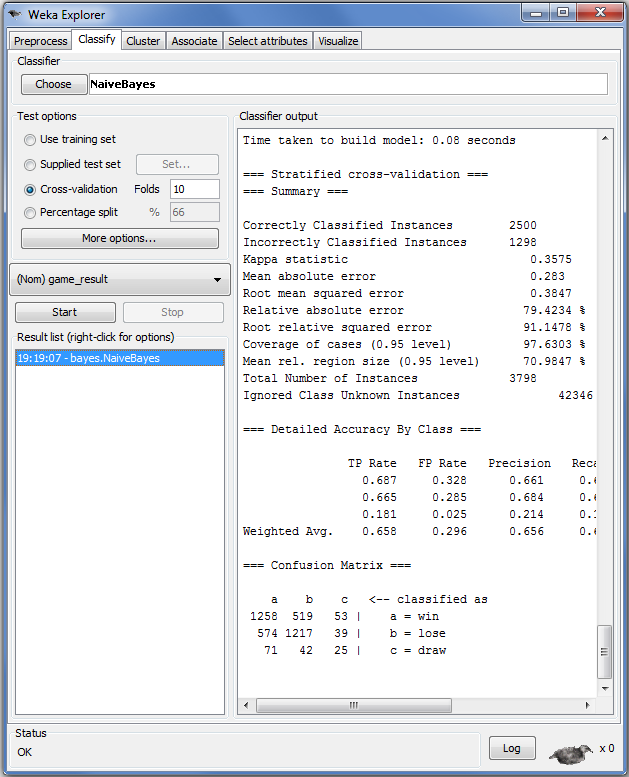
\includegraphics[width = 5.6in]{Screenshots/Weka.png}
\caption{A screenshot of the Weka Explorer.
%\\ useful for visualising ARFF files and trying out classifiers.
}
\label{screenshot:weka}
\end{figure}

The alternatives to using Weka would have been to create my own machine learning algorithms, which I did not have time to do, or to use a different software package, for example Matlab. In the end I chose to use Weka because it runs on Java, which is also used by \pap, and because it looked easy to use. 

Note that even though Weka produced the classifiers, I still had to write a significant amount of code to integrate them into the program.

Unfortunately, because \pa runs with Java 1.5, I was not able to use the most recent version of Weka and had to use an older version from 2004 (version 2.3.3). I doubt this had much of a negative effect on the project as version 2.3.3 had all the required features. 




\section{Training Data}							% ----

% Needed by Weka.
% Mention that game records are called hand histories.
% Originally intended to get it from a source on the web (cite them).
% Realised that I could just as easily get it by playing \sbt against itself in \pa.
% Still haven't looked at the online data.
% Also tried using data gathered by playing \sbt against \mbt once I had a working program. Didn't provide much of a difference.
% Mention the problem of converting the hh's into something that Weka can recognise.
% \pa exports and the internet hh's come in plain text human readable descriptions. 
% I planned to do it by writing a tool to convert them into arff.


In order for Weka to create a classifier, it needs to be provided with training data. In this case, training data takes the form of records of played games (called hand histories). I had originally planned to get hand histories from a source on the internet \cite{dataminedhhs}. I eventually realised that I could get hand histories more easily by playing \sbt against another instance of itself inside \pap. Early on in the project, I set up a match of \sbt Vs. \sbt and let it run for 50,000 games. I used that as the training data for all of the classifiers I created.

There is also a problem of converting the hand histories into a format that Weka can recognise. Hand histories exported from \pa (or from the web) come as human readable plain text descriptions of the games. Before I could use them as training data for Weka, I first had to convert them into Attribute Relation File Format (ARFF). I wrote my own tools to do this as there are no freely available ones. 
%I ended up spending a lot of time experimenting with different ways of representing the hand histories.



\section{The Plan}								% ----

% First the basic classes and logic.
% Next the \mcts algorithm.
% Next the opponent model.
% Explanation of why in that order.
% Explain about how you can easily change the strategies used.
% Mention the full original plan in the appendix.
% Evidence of good software practice?
% Something about design specifications?

% What I originally planned to do.
% Improving simulation and selection strategies.
% Improving the predictive capabilities of the opponent models.
% Adapt on the fly to new and different opponents. Not done because I didn't really have any different opponents to play against.

% Requirements analysis, or something else?

In my original plan, I proposed to complete the work in the following order:
\begin{enumerate}
\item Create the basic classes needed, implement the game logic and integrate with \pap.
\item Implement the framework for the MCTS algorithm and create basic strategies.
\item Implement more complex strategies for the MCTS algorithm. 
\item Collect and consolidate hand histories. 
\item Use Weka to create opponent models and integrate them into the main program.
\item Evaluation and testing. 
\end{enumerate}

%Part of the reason I chose to do it in this order was that it meant I would be able to have a working poker bot half way through the project. 

I chose to do it in this order because it allowed me to produce a working poker bot after the first term. It would have also allowed me to complete the project without the opponent model if the implementation of the MCTS algorithm had taken too long. 


Throughout the project, I was using Mercurial for version control and Dropbox to backup the repository. I had also intended to write good documentation for all of the classes in the project\footnote{However, due to time constraints, I was not always able to do this.}.



%If I had completed all of that and still had time to do more, I was going to attempt the following extensions:
%\begin{enumerate}
%\item Making the opponent models adapt to specific players on the fly.
%\item Try out some more elaborate simulation and selection strategies. 
%\item 
%\end{enumerate}

%In the end, I didn't have time to complete any of these. 

% TODO: add more?
























